\subsection{DONE}
\subsection{DONE}
\subsection{DONE}
\subsection{DONE}
\subsection{}
\subsubsection{DONE}
We fixed the front wheel to remove the singularity of K. $q_{\text{init}}$  was given as:

\begin{equation}\label{eq:4.5.1}
    \begin{split}
        q_{\text{init}} = 
        \begin{pmatrix}
            &\theta_{\text{Frame}} = 0\\
            &x_{\text{Frame}} = 0\\
            &y_{\text{Frame}} = 0.22\\
            &\theta_{\text{Wheel Back}} = 0\\
            % &\theta_{\text{Wheel Front}} = 0\\
            &\theta_{\text{Tire Front}} = 0\\
            &\theta_{\text{Tire Back}} = 0\\
            &y_{\text{Tire Front}} = 0.21\\
            &y_{\text{Tire Back}} = 0.21\\
            &\beta_{\text{Link Back}} = \pi\\
            &\beta_{\text{Link Front}} = 0
        \end{pmatrix}
    \end{split}
\end{equation}

Which represents this position:

\begin{figure}[ht]
    \centering
    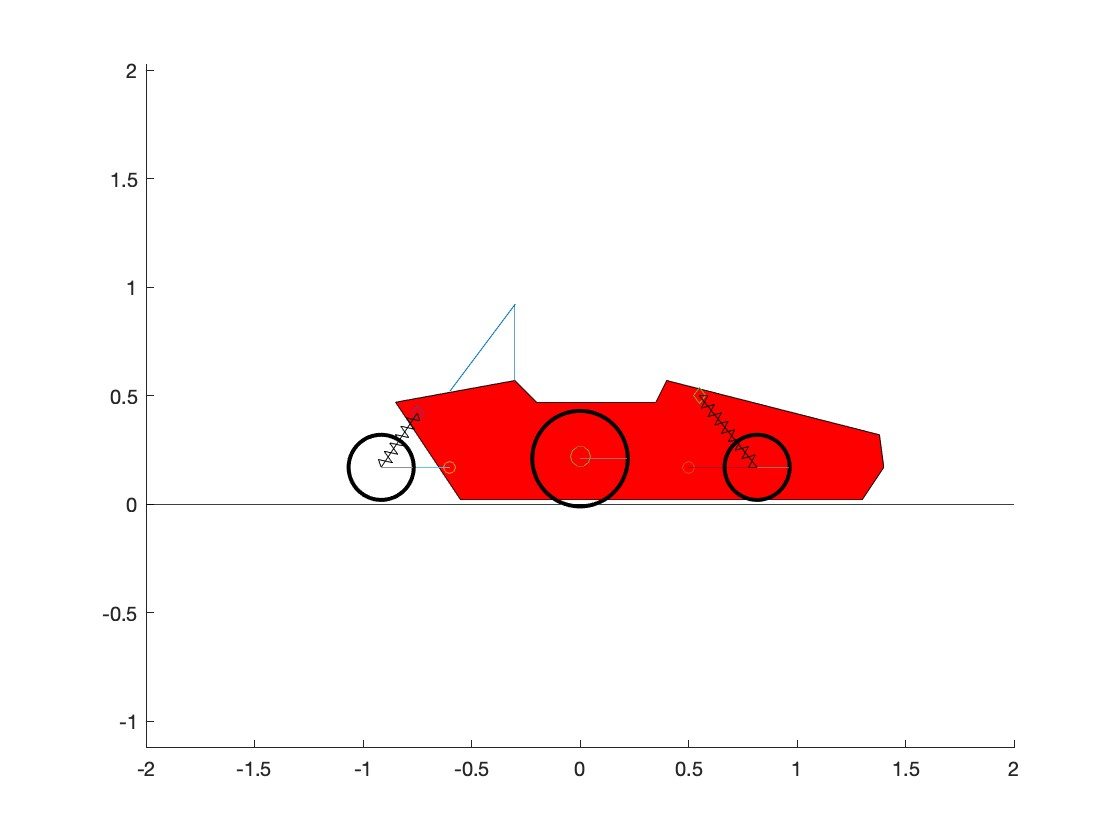
\includegraphics[scale=0.235]{images/q_init_1.jpg}
    \caption{Initial Position 1}
    %label always in the end
    \label{fig:init_1}
\end{figure}


This resulted in the equilibrium:

\begin{equation}\label{eq:4.5.2}
    \begin{split}
        q_{\text{equilibrium 1}} = 
        \begin{pmatrix}
            &\theta_{\text{Frame}} = -1.3896e-02 = -0.014\\
            &x_{\text{Frame}} =  -8.1104e-01 = -0.811\\
            &y_{\text{Frame}} = 2.1926e-01 = -0.219\\
            &\theta_{\text{Wheel Back}} = 7.8437e+00 = 7.844\\
            % &\theta_{\text{Wheel Front}} = 0\\
            &\theta_{\text{Tire Front}} = 2.2254e-21 \approx 0\\
            &\theta_{\text{Tire Back}} = 7.8437e+00 = 7.844\\
            &y_{\text{Tire Front}} = 2.1883e-01 = 0.219\\
            &y_{\text{Tire Back}} = 2.1895e-01 = 0.219\\
            &\beta_{\text{Link Back}} = 3.0209e+00 = 3.021\\
            &\beta_{\text{Link Front}} = 1.6787e-01 = 0.168
        \end{pmatrix}
    \end{split}
\end{equation}
Which is visualized by this figure:

\begin{figure}[ht]
    \centering
    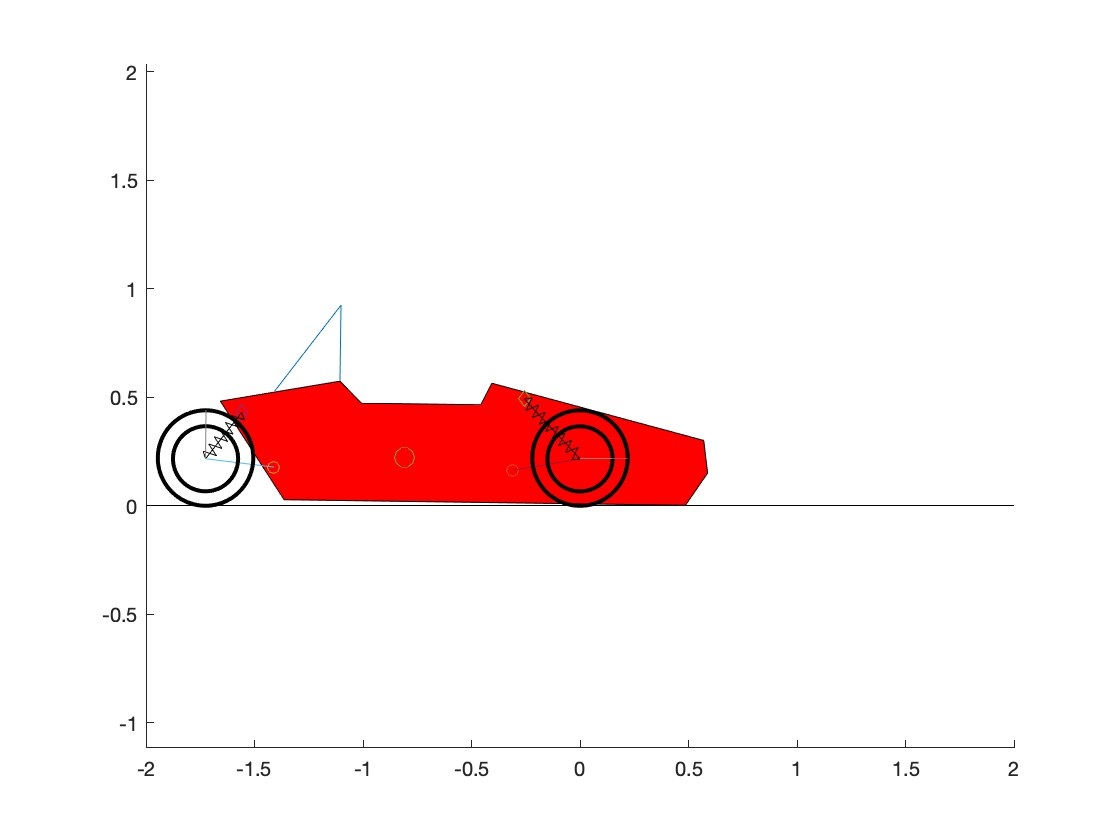
\includegraphics[scale=0.235]{images/Equilibrium1.jpg}
    \caption{Equilibrium Position 1}
    %label always in the end
    \label{fig:eq_1}
\end{figure}

\noindent In this example the choice of initial generalized coordinates was obviously very good. For the first task of this assignment the goal is to find two more (probably bad) equilibria.



\subsubsection{Different Equilibrium states}

The first alternative is luckily already given in the code. Again we fix the front wheel's rotation and start with the initial state:

\begin{equation}\label{eq:4.5.3}
    \begin{split}
        q_{\text{init}} = 
        \begin{pmatrix}
            &\theta_{\text{Frame}} = \pi/2\\
            &x_{\text{Frame}} = 0\\
            &y_{\text{Frame}} = 90\\
            &\theta_{\text{Wheel Back}} = 0\\
            % &\theta_{\text{Wheel Front}} = 0\\
            &\theta_{\text{Tire Front}} = 0\\
            &\theta_{\text{Tire Back}} = 0\\
            &y_{\text{Tire Front}} = 1.90\\
            &y_{\text{Tire Back}} = 0.21\\
            &\beta_{\text{Link Back}} = -\pi/2\\
            &\beta_{\text{Link Front}} = \pi/2
        \end{pmatrix}
    \end{split}
\end{equation}

Which represents this position:


\begin{figure}[ht]
    \centering
    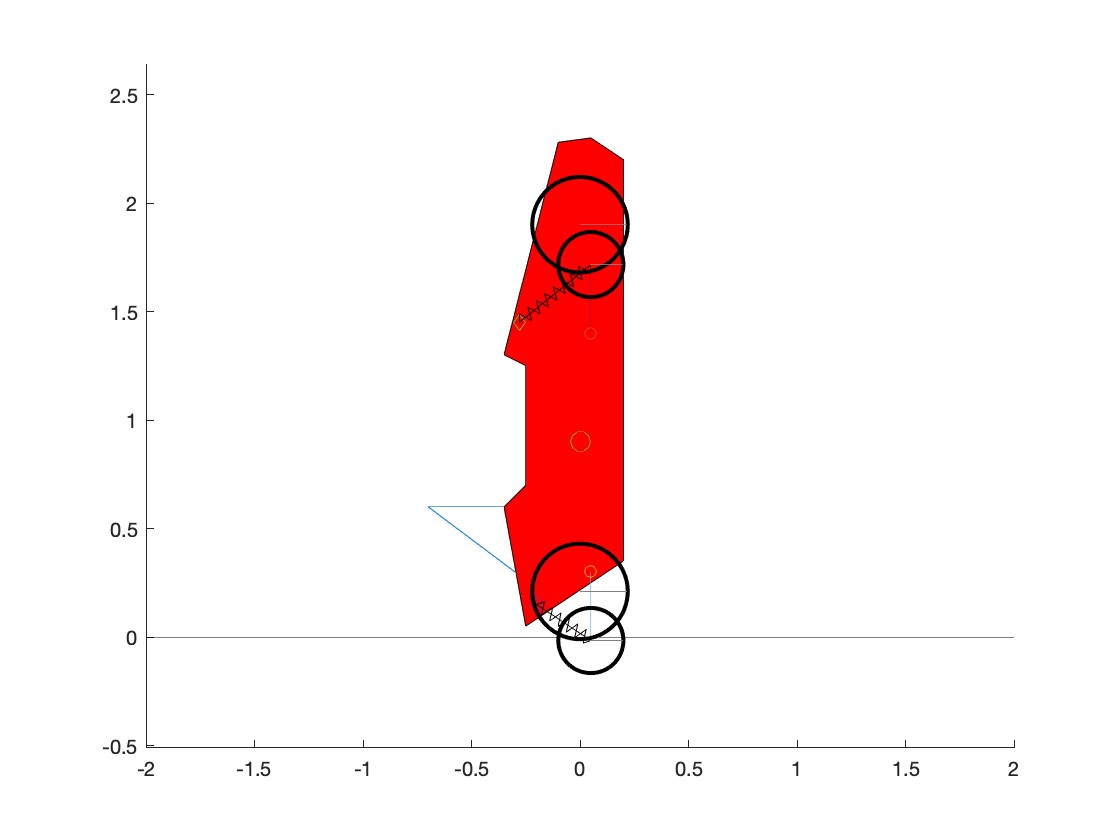
\includegraphics[scale=0.235]{images/q_init_2.jpg}
    \caption{Initial Position 2}
    %label always in the end
    \label{fig:init_2}
\end{figure}
\noindent Note: in the code provided $\theta_{\text{Frame}}$ was $\pi$ which was a different initial set of gen. coord. but converged to the same solution\\
\vspace{2mm}

\noindent As can be seen, this is obviously not a good choice of initial coordinates.

This setting converges to:

\begin{equation}\label{eq:4.5.4}
    \begin{split}
        q_{\text{init}} = 
        \begin{pmatrix}
            &\theta_{\text{Frame}} = 1.5248e+00\\
            &x_{\text{Frame}} = -6.9703e-02\\
            &y_{\text{Frame}} = 1.1280e+00\\
            &\theta_{\text{Wheel Back}} = 3.0427e-01\\
            % &\theta_{\text{Wheel Front}} = 0\\
            &\theta_{\text{Tire Front}} = 2.9622e-24\\
            &\theta_{\text{Tire Back}} = 3.0427e-01\\
            &y_{\text{Tire Front}} = 1.9414e+00\\
            &y_{\text{Tire Back}} = 2.1777e-01\\
            &\beta_{\text{Link Back}} = -1.6327e+00\\
            &\beta_{\text{Link Front}} = 1.5811e+00
        \end{pmatrix}
    \end{split}
\end{equation}

Which looks as follows:

\begin{figure}[ht]
    \centering
    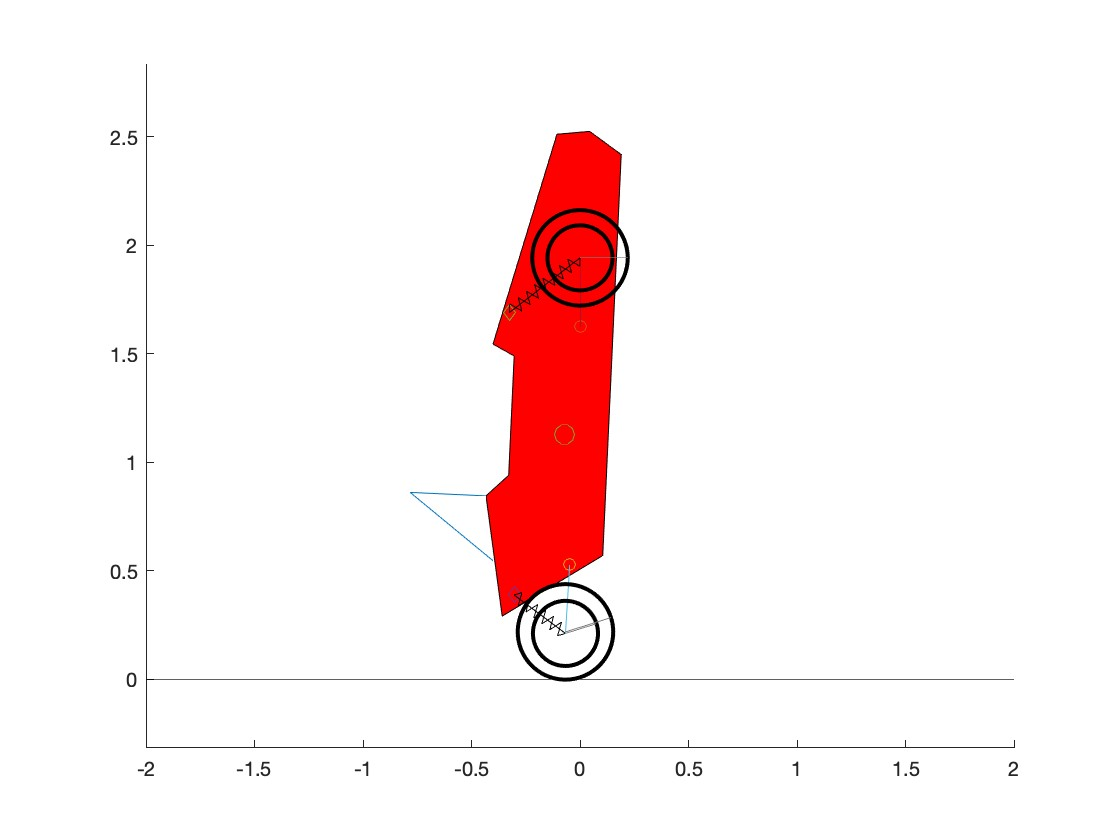
\includegraphics[scale=0.235]{images/Equilibrium2.jpg}
    \caption{Equilibrium Position 2}
    %label always in the end
    \label{fig:eq_2}
\end{figure}

The code example which has even worse initial conditions:

\begin{equation}\label{eq:4.5.5}
    \begin{split}
        q_{\text{init}} = 
        \begin{pmatrix}
            &\theta_{\text{Frame}} = \pi\\
            &x_{\text{Frame}} = 0\\
            &y_{\text{Frame}} = 90\\
            &\theta_{\text{Wheel Back}} = 0\\
            % &\theta_{\text{Wheel Front}} = 0\\
            &\theta_{\text{Tire Front}} = 0\\
            &\theta_{\text{Tire Back}} = 0\\
            &y_{\text{Tire Front}} = 1.90\\
            &y_{\text{Tire Back}} = 0.21\\
            &\beta_{\text{Link Back}} = -\pi/2\\
            &\beta_{\text{Link Front}} = \pi/2
        \end{pmatrix}
    \end{split}
\end{equation}

And looks like this:

\begin{figure}[ht]
    \centering
    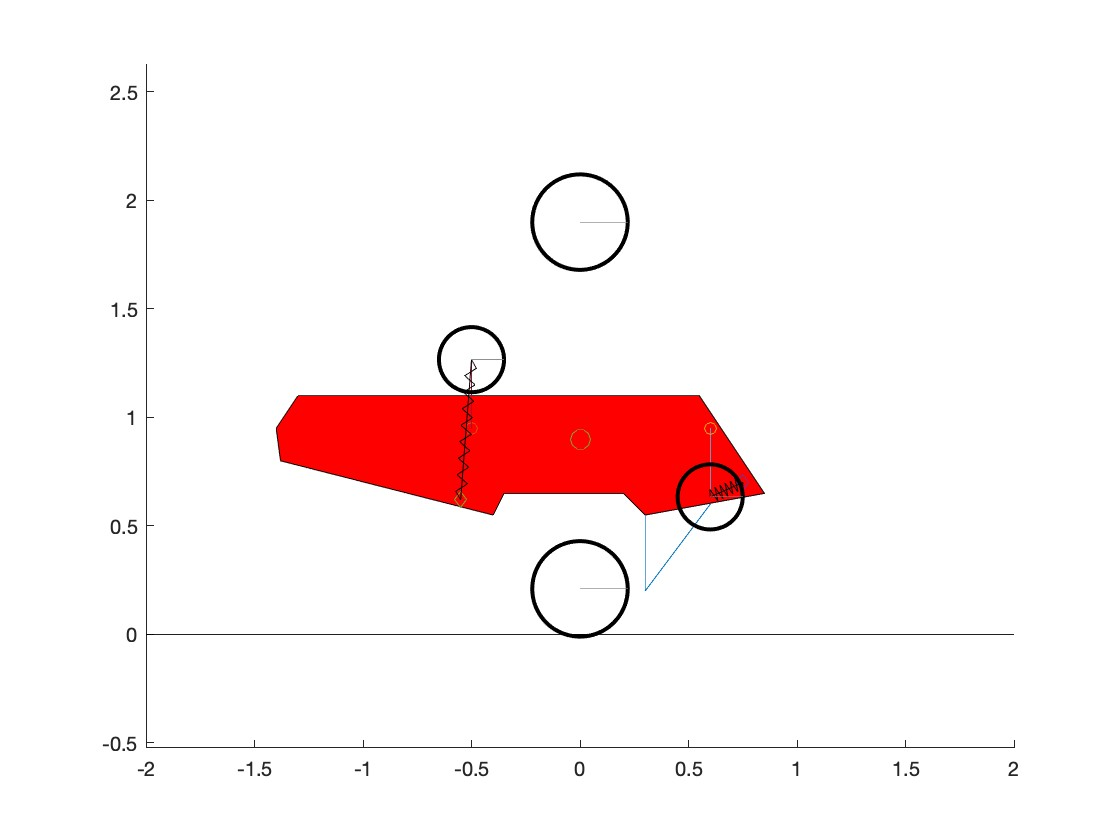
\includegraphics[scale=0.235]{images/q_init_3.jpg}
    \caption{Initial Position 3}
    %label always in the end
    \label{fig:init_3}
\end{figure}

Converges to:

\begin{equation}\label{eq:4.5.6}
    \begin{split}
        q_{\text{init}} = 
        \begin{pmatrix}
            &\theta_{\text{Frame}} = 2.0225e+00\\
            &x_{\text{Frame}} =  -1.2734e-01\\
            &y_{\text{Frame}} = 6.3440e-01\\
            &\theta_{\text{Wheel Back}} = 5.5591e-01\\
            % &\theta_{\text{Wheel Front}} = 0\\
            &\theta_{\text{Tire Front}} =  2.0275e-25\\
            &\theta_{\text{Tire Back}} = 5.5591e-01\\
            &y_{\text{Tire Front}} = 1.2043e+00\\
            &y_{\text{Tire Back}} = 2.1777e-01\\
            &\beta_{\text{Link Back}} = -3.4446e+00\\
            &\beta_{\text{Link Front}} = 3.1586e-01
        \end{pmatrix}
    \end{split}
\end{equation}
\clearpage%HERE
Which represents:

\begin{figure}[ht]
    \centering
    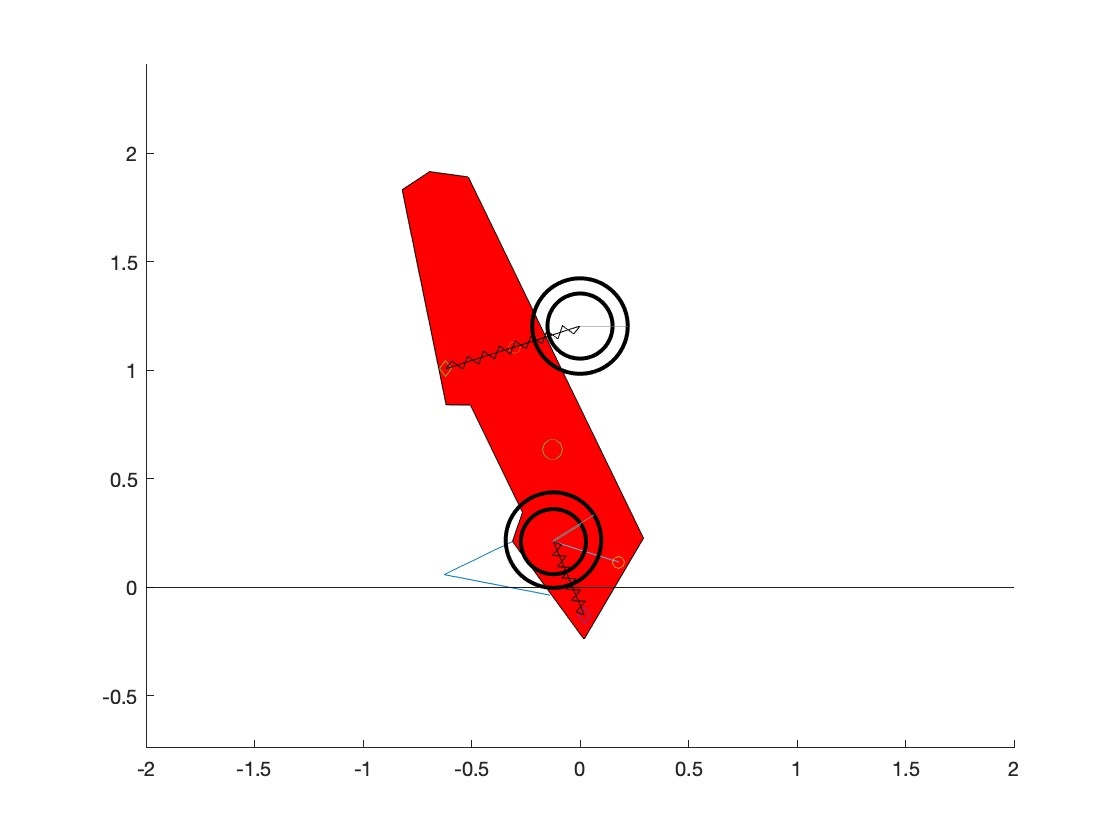
\includegraphics[scale=0.235]{images/Equilibrium3.jpg}
    \caption{Equilibrium Position 3}
    %label always in the end
    \label{fig:eq_3}
\end{figure}

\subsection{Analysis}
As we are working with a first order linearization of the dynamics of the system we have to stay in the proximity of the desired state of convergence. So a horizontal car with the initial conditions as seen in equation \ref{eq:4.5.1} will converge to a reasonable solution. \\\vspace{3mm}

\noindent Initial conditions like a 90° or 180° rotation of the frame can converge to a local solution as seen in Figure \ref*{fig:eq_3}\\\vspace{3mm}

\noindent The equilibrium from figure \ref{fig:eq_1} surely is stable as we all know it from reality. The two alternatives however are not stable. This can be seen from the example in fig \ref{fig:init_4} when the angle of the frame is between 0 and 90°:

\begin{figure}[ht]
    \centering
    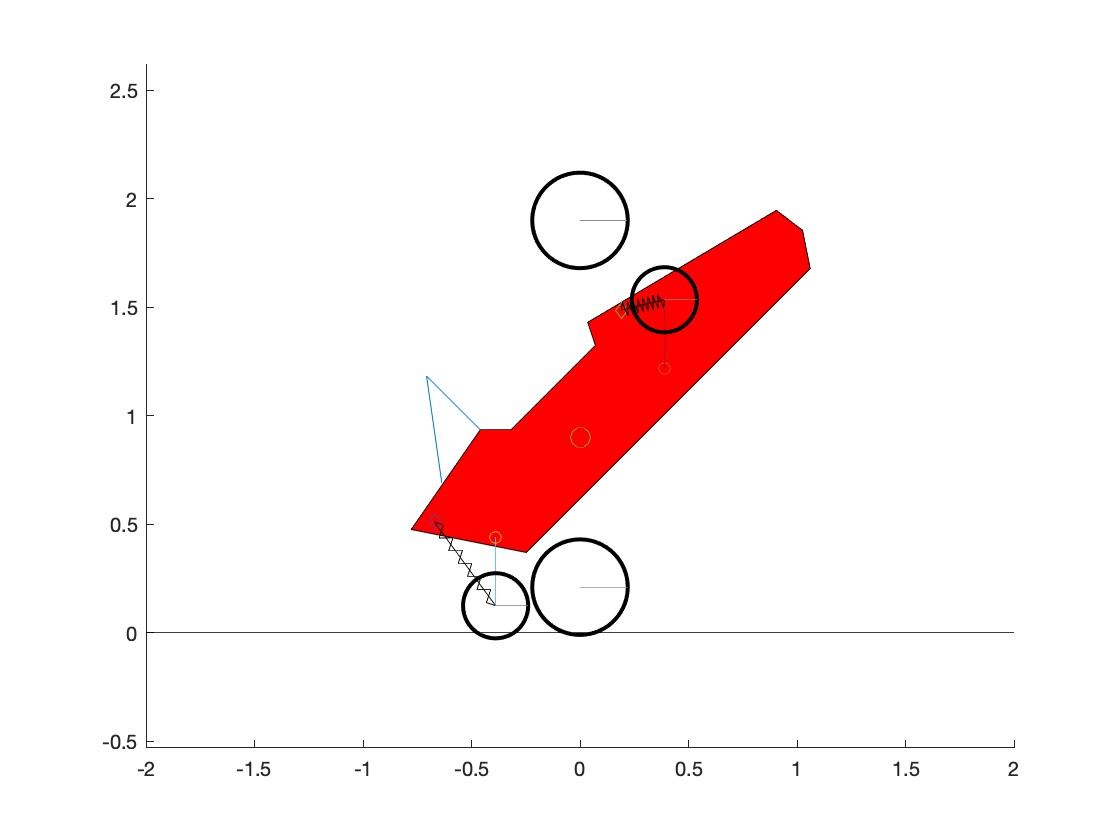
\includegraphics[scale=0.235]{images/q_init_4.jpg}
    \caption{Initial Position 4}
    %label always in the end
    \label{fig:init_4}
\end{figure}

Which converges to 

\begin{figure}[ht]
    \centering
    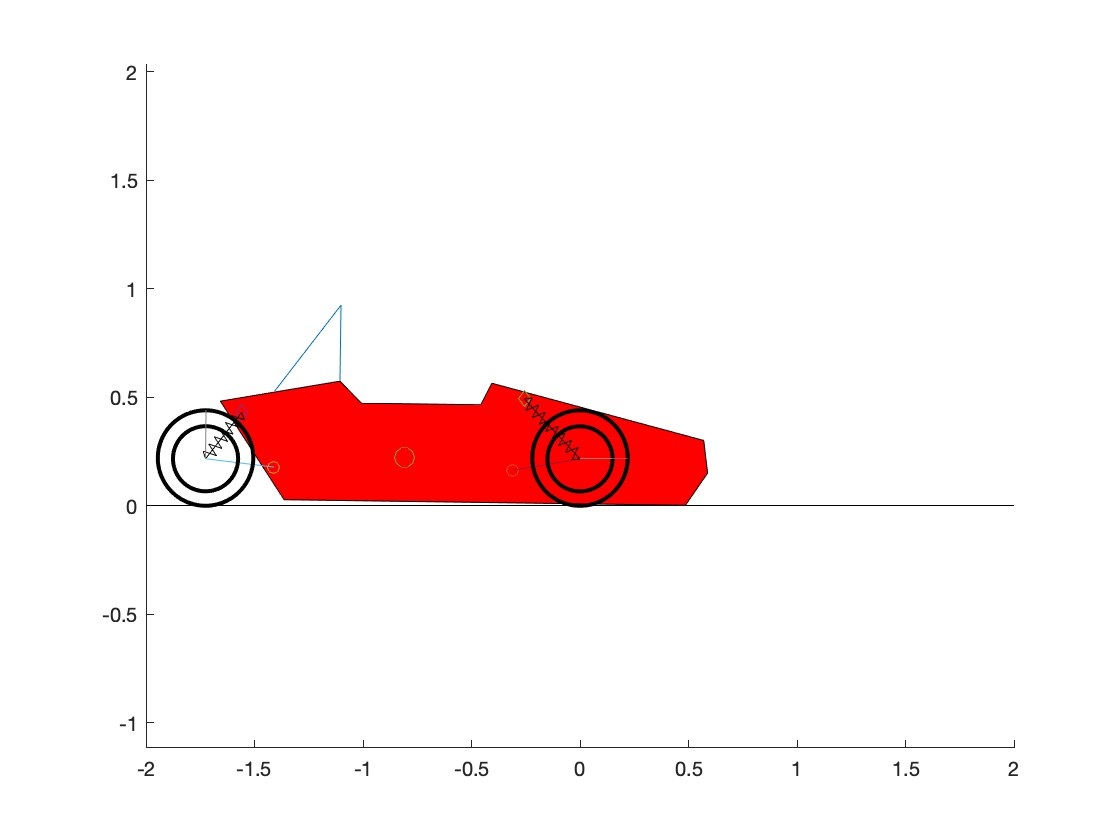
\includegraphics[scale=0.235]{images/Equilibrium4.jpg}
    \caption{Equilibrium Position 4}
    %label always in the end
    \label{fig:eq_4}
\end{figure}

So as we can see even with nonsensical other parameters when rotating the frame a bit less than 90° we converge to the stable solution.

\subsection{DONE}
\subsection{Eigenmodes and Eigenfrequencies}
\subsubsection{DONE}
\subsubsection{Mode Shapes}